\chapter{Perancangan Perangkat Lunak}
\label{chap:perancangan}

Pada bab ini akan dijabarkan perancangan perangkat lunak untuk penelitian ini. Perancangan perangkat lunak tersebut meliputi perancangan antarmuka dan perancangan kelas untuk penelitian ini.

\section{Perancangan Antarmuka}
\label{sec:antarmuka}

Perancangan antarmuka yang dibuat disesuaikan dengan diagram kelas dan diagram aktivitas yang dibuat sesuai analisis perangkat lunak dilakukan. Rancangan antarmuka dapat dilihat pada Gambar~\ref{fig:tab-rrp}. Pada bagian atas antarmuka terdapat sebuah kolom untuk memasukkan dokumen berjenis \textit{comma-separated values} yang ingin diacak. Pertama-tama pengguna wajib untuk mengisi kolom tersebut apapun teknik \textit{Randomization} yang akan digunakan nanti. Setelah pengguna memasukkan dokumen yang diinginkan, perangkat lunak akan menampilkan berbagai informasi mengenai dataset yang ada di dokumen tersebut seperti ukuran dokumen, nama dokumen, dan jumlah kolom. Deskripsi ini bertujuan untuk memberitahukan pengguna bahwa dokumen yang dimasukkan telah benar dan bagaimana sifat dari dataset yang dimasukkan. Pengguna juga sekarang harus memilih teknik mana yang ingin digunakan. Tampilan antarmuka akan menyesuaikan secara otomatis sesuai teknik yang dipilih dan dapat dilihat perubahannya pada Gambar~\ref{fig:tab-rpp} apabila teknik \textit{Random Projection Perturbation} yang dipilih.

\begin{figure}
	\centering
	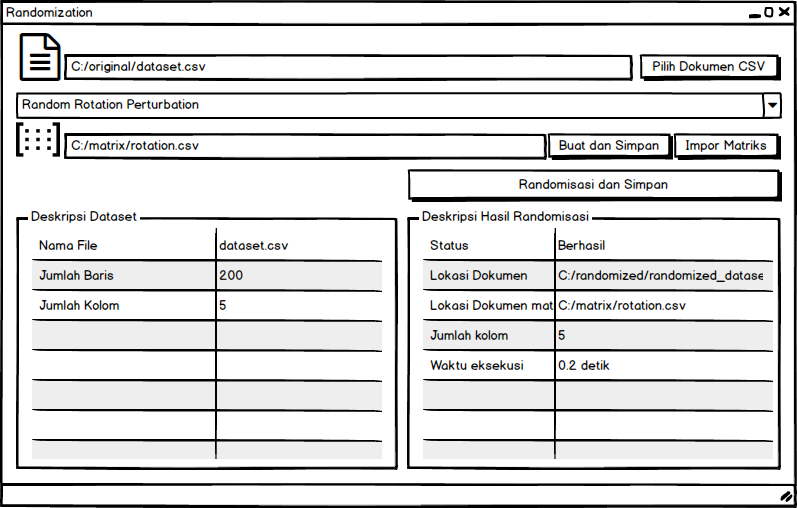
\includegraphics[scale=0.56]{tab-rrp}
	\caption{Halaman saat memilih teknik \textit{Random Rotation Perturbation}}
	\label{fig:tab-rrp}
\end{figure}

\begin{figure}
	\centering
	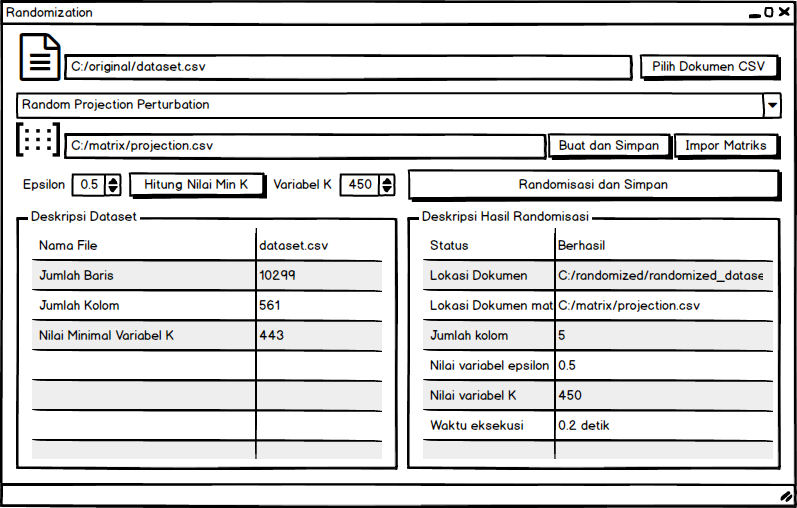
\includegraphics[scale=0.56]{tab-rpp}
	\caption{Halaman saat memilih teknik \textit{Random Projection Perturbation}}
	\label{fig:tab-rpp}
\end{figure}

Sebelum melakukan metode \textit{Randomization}, pengguna perlu memilih untuk membuat matriks rotasi/proyeksi baru atau mengiimpor matriks rotasi/proyeksi yang sudah pernah dibuat masing-masing dengan menekan tombol "Buat dan Simpan" dan "Impor Matriks". Pada teknik \textit{Random Projection Perturbation}, ada persyaratan yang harus dipenuhi mengenai dimensi akhir yang diinginkan dan nilai Epsilon. Kedua nilai tersebut perlu sesuai dengan dataset yang ada sehingga pengguna tidak bisa sembarangan menentukan dimensi dan nilai Epsilon. Perangkat lunak akan membuat aturan mengenai minimal dimensi yang bisa digunakan sehingga pengguna tidak bisa memasukan dimensi yang lebih kecil dari minimal yang telah ditentukan.

Setelah pengguna melakukan berbagai pengaturan, pengguna dapat melakukan pengacakan dengan menekan tombol \textquotedblleft Acak dan Simpan\textquotedblright. Apabila pengacakan berhasil dilakukan, perangkat lunak akan menampilkan \textit{popup} yang memberitahukan bahwa pengacakan berhasil dilakukan. \textit{Popup} tersebut dapat dilihat pada Gambar~\ref{fig:popup-sukses}. Selain itu, perangkat lunak juga akan menampilkan berbagai informasi beserta deskripsi tentang hasil pengacakan yang berhasil dilakukan.

\begin{figure}
	\centering
	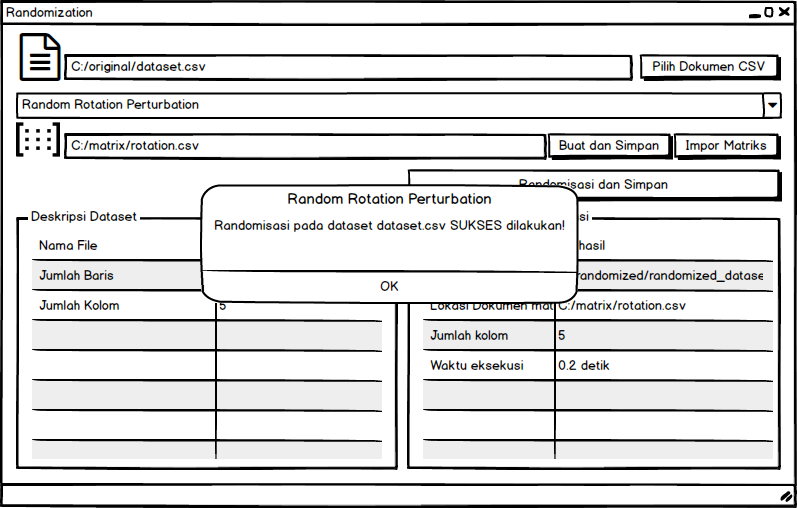
\includegraphics[scale=0.56]{popup-sukses}
	\caption{\textit{Popup} yang ditampilkan apabila pengacakan sukses dilakukan}
	\label{fig:popup-sukses}
\end{figure}

Perangkat lunak akan menampilkan deskripsi hasil dari pengacakan yang dilakukan. Informasi yang ditampilkan oleh perangkat lunak antara lain nama dokumen, ukuran dokumen, jumlah fitur, nilai Epsilon yang dipakai, jumlah dimensi pada hasil pengacakan, dan kolom yang diabaikan. Informasi ini ditampilkan oleh perangkat lunak bertujuan untuk memberitahukan pengguna properti-properti dataset yang telah diacak dan pengguna dapat memeriksa hasil yang dihasilkan oleh perangkat lunak apakah sesuai dengan keinginan pengguna.

Apabila ada masalah-masalah tertentu dan pengacakan gagal dilakukan, maka perangkat lunak akan memberitahukan bahwa pengacakan telah gagal dilakukan dengan menampilkan \textit{popup} yang berisi peringatan bahwa pengacakan gagal dilakukan. Hasil pengacakan tidak akan terbuat dan perangkat lunak akan menampilkan informasi bahwa metode \textit{Randomization} gagal dilakukan. \textit{Popup} tersebut dapat dilihat pada Gambar~\ref{fig:popup-gagal}. Oleh karena adanya persyaratan yang harus dipenuhi oleh pengguna untuk melakukan pengacakan dengan teknik \textit{Random Projection Perturbation}, maka pengacakan bisa saja gagal dilakukan karena persyaratan yang ada tidak dipenuhi oleh pengguna. Persyaratan yang disebutkan adalah persyaratan jumlah dimensi dan nilai Epsilon yang telah dijelaskan di atas. Perangkat lunak akan menampilkan \textit{popup} yang memberitahukan bahwa persyaratan tidak dipenuhi dan pengguna harus mengatur kembali pengaturan atau mengganti dataset. Rancangan ini dapat dilihat pada Gambar~\ref{fig:popup-syarat}.

\begin{figure}
	\centering
	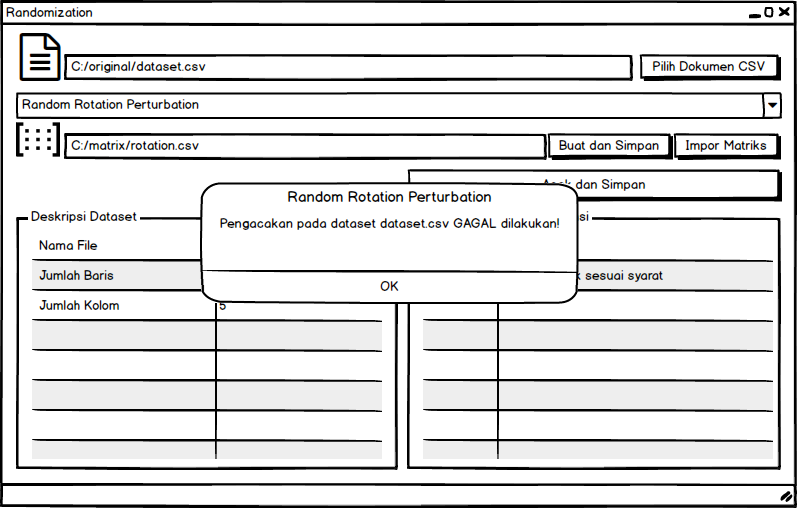
\includegraphics[scale=0.56]{popup-gagal}
	\caption{\textit{Popup} yang ditampilkan apabila pengacakan gagal dilakukan}
	\label{fig:popup-gagal}
\end{figure}

\begin{figure}
	\centering
	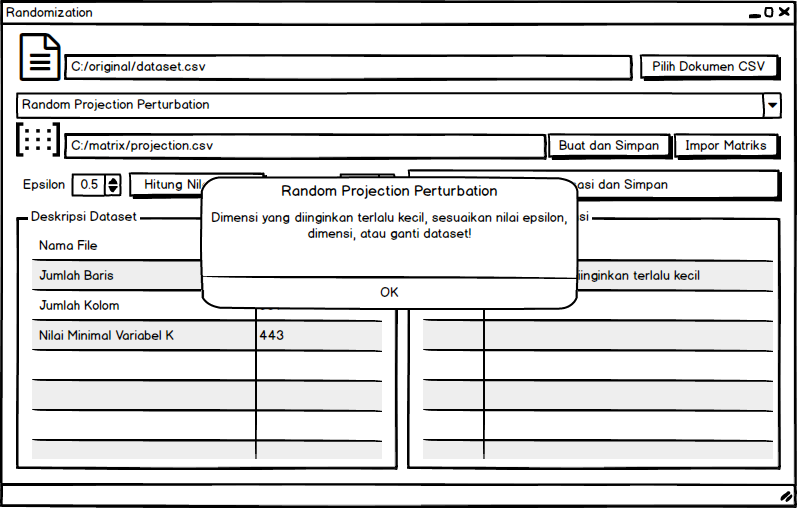
\includegraphics[scale=0.56]{popup-syarat}
	\caption{\textit{Popup} yang akan ditampilkan apabila persyaratan pada dataset tidak terpenuhi}
	\label{fig:popup-syarat}
\end{figure}

\section{Perancangan Kelas}
\label{sec:kelas}

Dalam pengembangan perangkat lunak, perlu adanya perancangan perangkat lunak secara menyeluruh untuk menghindari kesulitan dan kebingungan pada waktu pengembangan. Perangkat lunak yang akan dibuat pada penelitian ini akan berorientasi objek sehingga perlu adanya perancangan kelas-kelas yang akan dibuat. Pada subbab ini akan dijelaskan perancangan kelas perangkat lunak dan apa saja kegunaannya.

\subsection{Diagram \textit{Package}}
\label{subsec:diagram-package}

Perangkat lunak akan mempunyai 4 buah \textit{package} yaitu \textit{Perturbation}, \textit{Matrix}, \textit{Preprocessor}, dan \textit{View}. Keempat \textit{package} ini mempunyai fungsinya masing-masing untuk mendukung perangkat lunak berjalan yang akan dijelaskan pada subbab ini. Diagram \textit{Package} perangkat lunak dapat dilihat pada Gambar~\ref{fig:packagediagram}

\begin{figure}
	\centering
	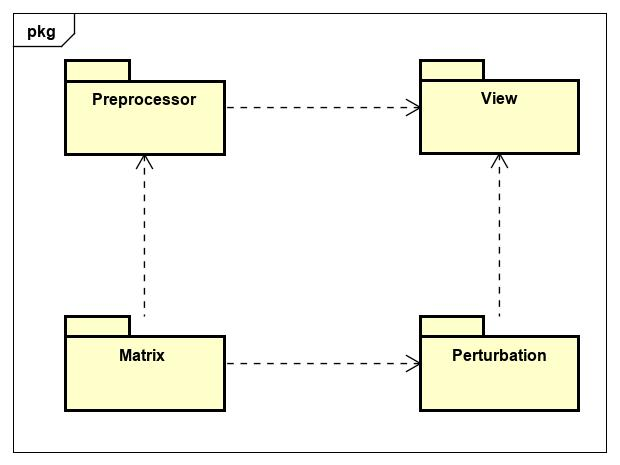
\includegraphics[scale=0.56]{packagediagram}
	\caption{Diagram \textit{package} perangkat lunak}
	\label{fig:packagediagram}
\end{figure}

\subsubsection{\textit{Package Perturbation}}
\label{subsubsec:package-perturbation}

\textit{Package Perturbation} merupakan \textit{package} yang menangani implementasi algoritma dari teknik \textit{Randomization} yang dipakai pada penelitian ini yaitu \textit{Random Rotation Perturbation} dan \textit{Random Projection Perturbation}. Kedua algoritma ini masing-masing akan menjadi sebuah kelas terpisah dan memiliki fungsinya masing-masing. Kedua kelas ini akan berada di dalam \textit{package Perturbation}. Satu kelas lagi akan ada di dalam \textit{package} ini yang berperan sebagai kelas \textit{super} bersifat abstrak untuk kedua kelas lainnya.

Dalam penerapan algoritma teknik yang dipakai, \textit{package} ini membutuhkan komponen atau fungsi lain untuk membuat algoritma yang diimplementasikan bekerja. Fungsi yang dibutuhkan antara lain adalah membuat matriks dengan sifat tertentu. Oleh karena itu \textit{package Perturbation} membutuhkan \textit{package Matrix} untuk membantu dalam pembuatan matriks yang khusus digunakan pada algoritma. \textit{Package Matrix} akan dijelaskan setelah ini.

\subsubsection{\textit{Package Matrix}}
\label{subsubsec:package-matrix}

\textit{Package Matrix} merupakan \textit{package} yang menangani segala jenis fungsi yang berkaitan dengan matriks. Semua fungsi yang terkait tentang matriks diimplementasikan pada \textit{package} ini, fungsi tersebut antara lain adalah implementasi struktur data matriks yang diimplementasikan pada sebuah kelas dan pembuatan matriks khusus yang akan dipakai untuk implementasi algoritma pada \textit{package Perturbation} yang diimplementasikan menjadi tiga buah kelas. \textit{Package} ini juga mengimplementasikan berbagai macam operasi matriks seperti perkalian, transpose matriks, dan menghitung determinan. Operasi-operasi ini diimplementasikan karena adanya kebutuhan operasi-operasi tersebut untuk membantu implementasi dari algoritma pada \textit{package Perturbation}.

\subsubsection{\textit{Package Preprocessor}}
\label{subsubsec:package-preprocessor}

\textit{Package Preprocessor} merupakan \textit{package} yang berfungsi sebagai \textit{preprocessor} untuk masukan dan keluaran perangkat lunak. Tentunya masukan yang diberikan pengguna kepada perangkat lunak tidak bisa langsung diolah begitu saja. Perlu adanya pengolahan terlebih dahulu sebelum masukan yang diterima dipakai pada perangkat lunak. Oleh karena itu, \textit{package} ini mempunyai fungsi untuk menyelesaikan masalah tersebut yaitu mengolah masukan yang diterima menjadi struktur data yang sesuai untuk digunakan pada perangkat lunak.

Pada penelitian ini, masukan perangkat lunak yang dimaksud adalah dataset yang akan diacak. Pengguna perlu mengikuti persyaratan masukan seperti apa yang dapat menjadi masukan perangkat lunak pada penelitian ini. Pada penelitian ini, perangkat lunak dirancang untuk hanya menerima dokumen berjenis \textit{comma-separated values}. Oleh karena itu, \textit{package preprocessor} ini memiliki sebuah fungsi untuk mengolah masukan berupa dokumen berjenis \textit{comma-separated values} menjadi struktur data matriks atau sebaliknya dengan menggunakan \textit{package Matrix}.

\subsubsection{\textit{Package View}}
\label{subsubsec:package-view}

\textit{Package View} merupakan \textit{package} yang menangani bagian antarmuka pada perangkat lunak di penelitian ini. Antarmuka perangkat lunak akan diimplementasikan menggunakan \textit{framework} antarmuka grafis berbasis bahasa pemograman Python yang bernama Kivy. \textit{Package} ini akan berisi kelas-kelas dan seluruh fungsi yang bertujuan untuk menampilkan antarmuka pada perangkat lunak.

\subsection{Diagram Kelas pada \textit{Package Perturbation}}
\label{subsec:diagram-kelas-perturbation}

\begin{figure}
	\centering
	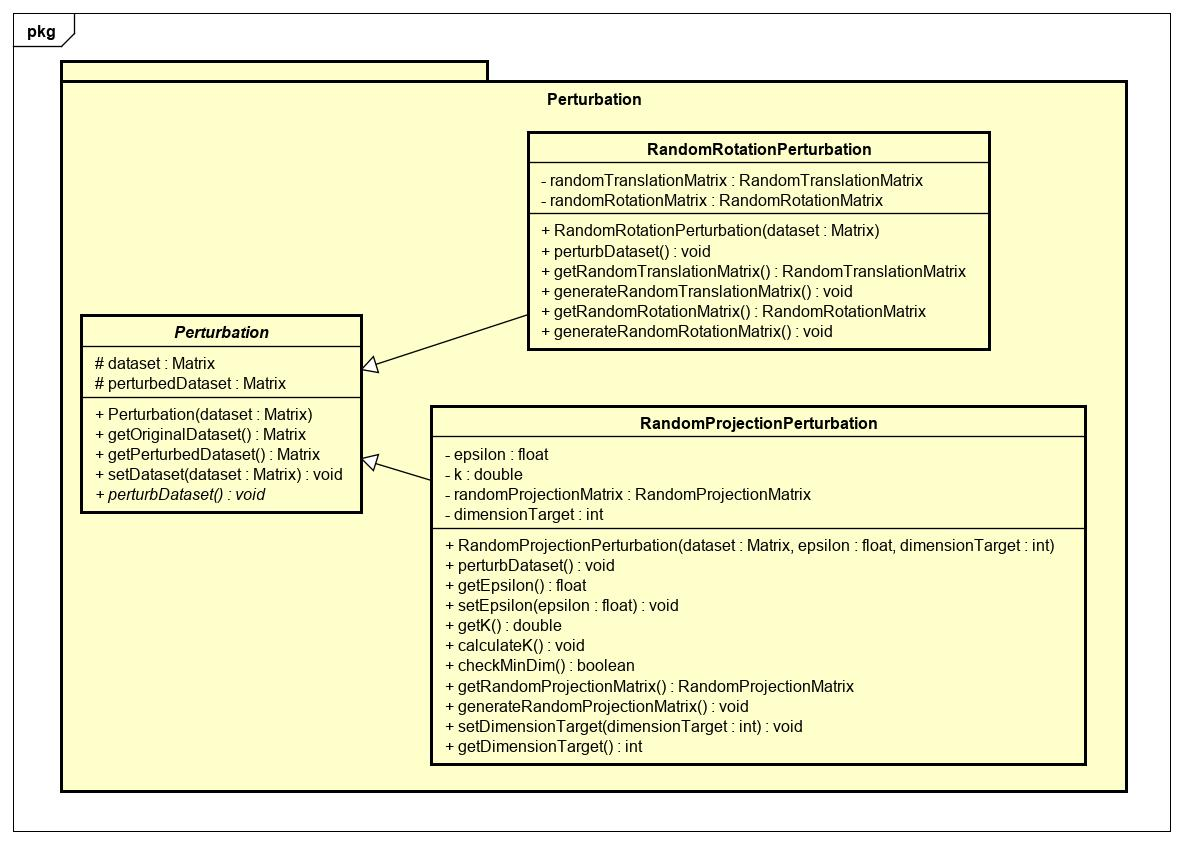
\includegraphics[scale=0.39]{perturbationclassdiagram}
	\caption{Diagram kelas pada \textit{package Perturbation}}
	\label{fig:perturbationclassdiagram}
\end{figure}

\textit{Package Perturbation} memiliki tiga buah kelas yang bertujuan untuk mengimplementasikan algoritma teknik \textit{Random Rotation Perturbation} dan \textit{Random Projection Perturbation}. Ketiga kelas tersebut adalah \textit{Perturbation}, \textit{RandomRotationPerturbation}, dan \textit{RandomProjectionPerturbation} yang akan dijelaskan secara detail pada subbab ini. Diagram kelas pada \textit{package Perturbation} dapat dilihat pada Gambar~\ref{fig:perturbationclassdiagram}.

\subsubsection{Kelas \textit{Perturbation}}
\label{subsubsec:kelas-perturbation}

Kelas \textit{Perturbation} berperan sebagai kelas abstrak yang akan menjadi kelas \textit{super} dari kedua kelas lainnya dalam package \textit{Perturbation} yaitu kedua kelas yang mengimplementasikan algoritma teknik \textit{Random Rotation Perturbation} dan \textit{Random Projection Perturbation}. Kelas ini mendeklarasikan atribut dan fungsi apa saja yang seharusnya diimplementasikan oleh kelas \textit{RandomRotationPerturbation}, dan \textit{RandomProjectionPerturbation}. Beberapa atribut dan fungsi tersebut masih kosong pada kelas \textit{Perturbation} sehingga berbagai atribut dan fungsi tersebut perlu didefinisikan pada kelas-kelas turunannya. Selanjutnya akan dijelaskan secara rinci tiap atribut dan fungsi pada kelas ini.

Berikut adalah deskripsi setiap atribut pada kelas \textit{Perturbation}.
\begin{itemize}
	\item \textit{dataset} adalah atribut untuk menampung dataset yang diambil dari masukan perangkat lunak yang ingin diacak dan sudah berbentuk matriks. Tipe data atribut ini adalah \textit{Matrix}.
	\item \textit{perturbedDataset} adalah atribut untuk menampung hasil dari dataset yang telah diacak. Tipe data atribut ini adalah \textit{Matrix}.
\end{itemize}

Berikut adalah deskripsi setiap fungsi pada kelas \textit{Perturbation}.
\begin{itemize}
	\item \textit{Perturbation} adalah \textit{constructor} dari kelas \textit{Perturbation}. Tujuan utama fungsi ini adalah mendefinisikan atribut-atribut yang ada. Fungsi ini memiliki sebuah masukan yang dinamakan \textit{dataset} yang bertipe data \textit{Matrix} dan berfungsi untuk mendefinisikan atribut \textit{dataset}.
	\item \textit{getOriginalDataset} adalah fungsi untuk mendapatkan dataset asli yang belum diacak atau dengan kata lain mendapatkan atribut \textit{dataset}. Fungsi ini tidak memiliki masukan apapun dan mempunyai tipe data kembalian berupa \textit{Matrix}.
	\item \textit{getPerturbedDataset} adalah fungsi untuk mendapatkan hasil dari dataset yang telah diacak atau dengan kata lain mendapatkan atribut \textit{perturbedDataset}. Fungsi ini tidak memiliki parameter apapun. Tipe data kembalian pada fungsi ini berupa \textit{Matrix}.
	\item \textit{setDataset} adalah fungsi untuk mendefinisikan ulang atribut \textit{dataset} dengan dataset yang baru. Fungsi ini memiliki sebuah masukan yang dinamakan \textit{dataset} yang bertipe data \textit{Matrix} dan berfungsi untuk mendefinisikan atribut \textit{dataset}. Tidak ada kembalian pada fungsi ini.
	\item \textit{perturbDataset} adalah fungsi untuk melakukan pengacakan pada atribut \textit{dataset} dan menyimpan hasilnya pada atribut \textit{perturbedDataset}. Fungsi ini bersifat abstrak yang berarti fungsi ini belum didefinisikan sehingga fungsi ini harus didefinisikan pada setiap kelas turunannya. Tidak ada kembalian ataupun masukan pada fungsi ini.
\end{itemize}

\subsubsection{Kelas \textit{RandomRotationPerturbation}}
\label{subsubsec:kelas-rrp}

Kelas \textit{RandomRotationPerturbation} adalah kelas yang mempunyai tujuan utama melakukan pengacakan dengan teknik \textit{Random Rotation Perturbation} pada dataset yang menjadi masukan perangkat lunak. Kelas ini merupakan kelas turunan dari kelas \textit{Perturbation} sehingga kelas inipun mewarisi semua atribut dan fungsi yang dimiliki oleh kelas \textit{Perturbation}. Oleh karena itu, fungsi \textit{perturbDataset} yang diturunkan dari kelas \textit{Perturbation} harus didefinisikan oleh kelas \textit{RandomRotationPerturbation}. Kelas ini akan mengimplementasikan algoritma dari teknik \textit{Random Rotation Perturbation} untuk melakukan pengacakan pada fungsi \textit{perturbDataset}. Selanjutnya akan dijelaskan secara rinci tiap atribut dan fungsi pada kelas ini.

Berikut adalah deskripsi setiap atribut pada kelas \textit{RandomRotationPerturbation}.
\begin{itemize}
	\item \textit{randomTranslationMatrix} adalah atribut untuk menampung matriks translasi yang akan dipergunakan untuk implementasi algoritma \textit{Random Rotation Perturbation}. Atribut ini mempunyai tipe data \textit{Matrix}.
	\item \textit{randomRotationMatrix} adalah atribut untuk menampung matriks rotasi yang akan dipergunakan untuk implementasi algoritma \textit{Random Rotation Perturbation}. Atribut ini mempunyai tipe data \textit{Matrix}.
\end{itemize}

Berikut adalah deskripsi setiap fungsi pada kelas \textit{RandomRotationPerturbation}.
\begin{itemize}
	\item \textit{RandomRotationPerturbation} adalah \textit{constructor} untuk mendefinisikan atribut-atribut yang ada dan memanggil \textit{constructor} dari kelas \textit{super} milik kelas \textit{RandomRotationPerturbation} yaitu \textit{Perturbation}. Tujuan utama fungsi ini adalah memanggil \textit{constructor} dari kelas \textit{super} yaitu \textit{Perturbation} sehingga fungsi ini berguna untuk mendefinisikan atribut \textit{dataset}. Selain itu, fungsi ini juga akan mendefinisikan atribut \textit{randomTranslationMatrix} dan \textit{randomRotationMatrix}.
	\item \textit{perturbDataset} adalah fungsi turunan dari kelas \textit{Perturbation} yang pada kelas \textit{RandomRotationPerturbation} diimplementasikan algoritma teknik \textit{Random Rotation Perturbation}. Fungsi ini akan mengimplementasikan algoritma teknik \textit{Random Rotation Perturbation} kepada atribut \textit{dataset} dan menyimpan hasilnya kepada atribut \textit{perturbedDataset}. Tidak ada masukan pada fungsi ini tetapi memiliki kembalian berupa \textit{boolean} yang menyatakan apakah pengacakan berhasil dilakukan.
	\item \textit{getRandomTranslationMatrix} adalah fungsi untuk mendapatkan matriks translasi yang digunakan untuk implementasi algoritma teknik \textit{Random Rotation Perturbation} atau dengan kata lain mendapatkan atribut \textit{randomTranslationMatrix}. Fungsi ini tidak memiliki masukan apapun tetapi mempunyai kembalian berupa matriks translasi yang bertipe data \textit{Matrix}.
	\item \textit{getRandomRotationMatrix} adalah fungsi untuk mendapatkan matriks rotasi yang digunakan untuk implementasi algoritma teknik \textit{Random Rotation Perturbation} atau dengan kata lain mendapatkan atribut \textit{randomRotationMatrix}. Fungsi ini tidak memiliki masukan apapun tetapi mempunyai kembalian berupa matriks rotasi yang bertipe data \textit{Matrix}.
\end{itemize}

\subsubsection{Kelas \textit{RandomProjectionPerturbation}}
\label{subsubsec:kelas-rpp}

Kelas \textit{RandomProjectionPerturbation} adalah kelas yang mempunyai tujuan utama melakukan pengacakan dengan teknik \textit{Random Projection Perturbation} pada dataset yang menjadi masukan perangkat lunak. Kelas ini merupakan kelas turunan dari kelas \textit{Perturbation} sehingga kelas inipun mewarisi semua atribut dan fungsi yang dimiliki oleh kelas \textit{Perturbation}. Oleh karena itu, fungsi \textit{perturbDataset} yang diturunkan dari kelas \textit{Perturbation} harus didefinisikan oleh kelas \textit{RandomProjectionPerturbation}. Kelas ini akan mengimplementasikan algoritma dari teknik \textit{Random Projection Perturbation} untuk melakukan pengacakan pada fungsi \textit{perturbDataset}. Selanjutnya akan dijelaskan secara rinci tiap atribut dan fungsi pada kelas ini.

Berikut adalah deskripsi setiap atribut pada kelas \textit{RandomProjectionPerturbation}.
\begin{itemize}
	\item \textit{epsilon} adalah atribut yang berguna untuk menentukan seberapa besar batas maksimal distorsi yang dapat terjadi pada hasil pengacakan. Atribut \textit{epsilon} ini akan digunakan untuk menghitung nilai dari atribut \textit{minK} yang akan dijelaskan nanti. Tipe data atribut ini adalah \textit{float}, bilangan riil yang nantinya hanya akan diisi dengan rentang nilai (0, 1). Pengguna akan menentukan seberapa besar batas maksimal distorsi yang dapat terjadi pada hasil pengacakan dengan cara mendefinisikan atribut \textit{epsilon} ini.
	\item \textit{minK} adalah atribut yang berguna untuk menentukan dimensi terkecil untuk sebuah dataset yang ingin diacak dapat direduksi dengan distorsi yang terkontrol sesuai atribut \textit{epsilon}. Atribut ini juga menentukan apakah dataset memenuhi persyaratan untuk direduksi yaitu memiliki jumlah kolom yang lebih besar dari nilai \textit{minK}. Tipe data atribut ini adalah \textit{double}, bilangan riil. Atribut ini akan dihitung oleh perangkat lunak sesuai nilai \textit{epsilon} yang telah ditentukan pengguna.
	\item \textit{k} adalah atribut untuk menyimpan besar dimensi akhir yang diinginkan pengguna dimiliki oleh hasil dataset yang telah diacak. Pengguna harus mendefinisikan atribut ini dengan nilai yang lebih besar dari atau sama dengan nilai \textit{minK}, jika tidak maka distorsi yang terjadi pada hasil pengacakan akan lebih besar dari nilai \textit{epsilon} yang diinginkan. Tipe data atribut ini adalah \textit{integer}, bilangan bulat.
\end{itemize}

Berikut adalah deskripsi setiap fungsi pada kelas \textit{RandomProjectionPerturbation}.
\begin{itemize}
	\item \textit{RandomProjectionPerturbation} adalah \textit{constructor} untuk mendefinisikan atribut-atribut yang ada dan memanggil \textit{constructor} dari kelas \textit{super} milik kelas \textit{RandomProjectionPerturbation} yaitu \textit{Perturbation}. Tujuan utama fungsi ini adalah memanggil \textit{constructor} dari kelas \textit{super} yaitu \textit{Perturbation} sehingga fungsi ini berguna untuk mendefinisikan atribut \textit{dataset}. Selain itu, fungsi ini juga akan mendefinisikan atribut \textit{epsilon}, \textit{minK}, dan \textit{k}.
	\item \textit{perturbDataset} adalah fungsi turunan dari kelas \textit{Perturbation} yang pada kelas \textit{RandomProjectionPerturbation} diimplementasikan algoritma teknik \textit{Random Projection Perturbation}. Fungsi ini akan mengimplementasikan algoritma teknik \textit{Random Projection Perturbation} kepada atribut \textit{dataset} dan menyimpan hasilnya kepada atribut \textit{perturbedDataset}. Tidak ada masukan pada fungsi ini tetapi memiliki kembalian berupa \textit{boolean} yang menyatakan apakah pengacakan berhasil dilakukan.
	\item \textit{getEpsilon} adalah fungsi untuk mendapatkan nilai batas maksimal distorsi yang dapat terjadi pada hasil pengacakan atau dengan kata lain mendapatkan atribut \textit{epsilon}. Fungsi ini tidak memiliki masukan apapun tetapi mempunyai kembalian berupa nilai dari atribut \textit{epsilon} yang bertipe data \textit{float}, bilangan riil.
	\item \textit{getMinK} adalah fungsi untuk mendapatkan besar dimensi minimal hasil dataset yang telah diacak atau dengan kata lain mendapatkan atribut \textit{minK}. Fungsi ini tidak memiliki masukan apapun tetapi mempunyai kembalian berupa nilai dari atribut \textit{minK} yang bertipe data \textit{double}, bilangan riil.
	\item \textit{calculateMinK} adalah fungsi untuk menghitung nilai \textit{minK} sesuai dengan atribut \textit{epsilon} dan jumlah baris pada dataset yang ingin diacak. Fungsi ini akan menghitung nilai \textit{minK} tersebut dan menyimpan hasilnya pada atribut \textit{minK}. Tidak ada masukan ataupun kembalian pada fungsi ini.
	\item \textit{checkMinK} adalah fungsi untuk memeriksa apakah dimensi dari \textit{dataset} yang ingin diacak lebih besar dari nilai \textit{minK}, besar dimensi minimal. Selain itu, fungsi ini memeriksa apakah nilai \textit{k} lebih besar dari atau sama dengan nilai \textit{minK}. Intinya fungsi ini menguji apakah dataset dan keinginan pengguna memenuhi persyaratan untuk mengaplikasikan teknik \textit{Random Projection Perturbation}. Fungsi ini tidak memiliki masukan apapun tetapi mempunyai kembalian berupa sebuah \textit{boolean} yang menandakan apakah \textit{dataset} dan \textit{k} yang diberikan oleh pengguna memenuhi persyaratan untuk mengaplikasikan teknik \textit{Random Projection Perturbation} dengan \textit{dataset} dan \textit{k} tersebut.
	\item \textit{checkVariableK} adalah fungsi untuk memeriksa apakah nilai \textit{k} lebih besar dari atau sama dengan nilai \textit{minK}. Fungsi ini tidak memiliki masukan apapun tetapi mempunyai kembalian berupa sebuah \textit{boolean} yang menandakan apakah nilai variabel \textit{k} yang diberikan oleh pengguna memenuhi persyaratan untuk mengaplikasikan teknik \textit{Random Projection Perturbation} dengan nilai variabel \textit{k} tersebut.
\end{itemize}

\subsection{Diagram Kelas pada \textit{Package Matrix}}
\label{subsec:diagram-kelas-matrix}

\begin{figure}
	\centering
	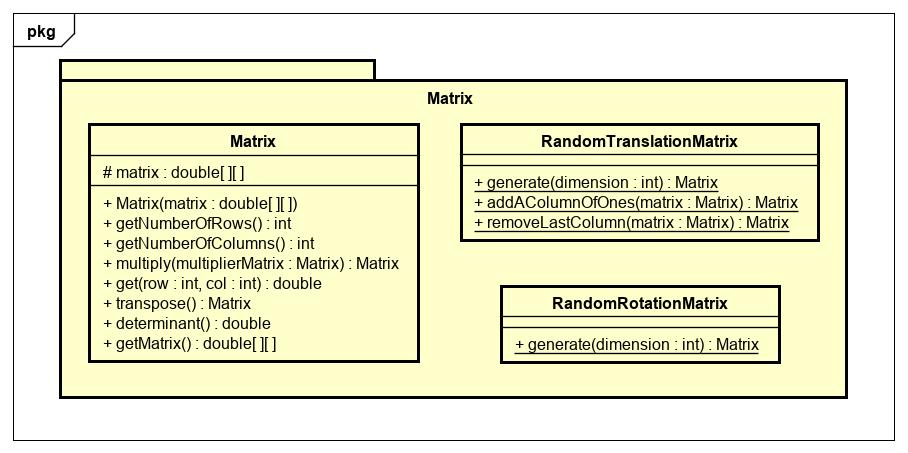
\includegraphics[scale=0.45]{matrixclassdiagram}
	\caption{Diagram kelas pada \textit{package Matrix}}
	\label{fig:matrixclassdiagram}
\end{figure}

\textit{Package Matrix} memiliki empat buah kelas yang bertujuan untuk menangani segala jenis fungsi yang berkaitan dengan matriks maupun pembuatan matriks yang khusus digunakan untuk implementasi algoritma. Keempat kelas tersebut adalah \textit{Matrix}, \textit{RandomTranslationMatrix}, dan \textit{RandomRotationMatrix} yang akan dijelaskan secara detail pada subbab ini. Diagram kelas pada \textit{package Matrix} dapat dilihat pada Gambar~\ref{fig:matrixclassdiagram}.

\subsubsection{Kelas \textit{Matrix}}
\label{subsubsec:kelas-matrix}

Kelas \textit{Matrix} adalah kelas yang menangani struktur data matriks serta segala fungsi atau operasi yang berkaitan dengan matriks. Kelas ini akan mempunyai semua kebutuhan terkait dengan urusan struktur data matriks yang ada untuk implementasi algoritma \textit{Random Rotation Perturbation} dan \textit{Random Projection Perturbation}, antara lain seperti perkalian, transpose matriks, dan mencari determinan. Selanjutnya akan dijelaskan secara rinci tiap atribut dan fungsi pada kelas ini.

Berikut adalah deskripsi setiap atribut pada kelas \textit{Matrix}.
\begin{itemize}
	\item \textit{matrix} adalah atribut untuk menyimpan matriks dengan cara menyimpannya memakai \textit{array} 2 dimensi dengan tipe data \textit{double}, bilangan riil.
\end{itemize}

Berikut adalah deskripsi setiap fungsi pada kelas \textit{Matrix}.
\begin{itemize}
	\item \textit{Matrix} adalah \textit{constructor} dari kelas \textit{PerturbMatrixation}. Tujuan utama fungsi ini adalah mendefinisikan atribut-atribut yang ada. Fungsi ini memiliki sebuah masukan berbentuk array yang dinamakan \textit{matrix} yang bertipe data \textit{double} dan berfungsi untuk mendefinisikan atribut \textit{matrix}.
	\item \textit{getNumberOfRows} adalah fungsi untuk mendapatkan jumlah baris yang ada pada matriks kelas ini atau dengan kata lain mendapatkan ukuran dari atribut \textit{matrix}. Fungsi ini tidak memiliki masukan apapun tetapi mempunyai kembalian berupa jumlah baris yang bertipe data \textit{integer}, bilangan bulat.
	\item \textit{getNumberOfColumns} adalah fungsi untuk mendapatkan jumlah kolom yang ada pada matriks kelas ini atau dengan kata lain mendapatkan ukuran dari atribut \textit{matrix}. Fungsi ini tidak memiliki masukan apapun tetapi mempunyai kembalian berupa jumlah baris yang bertipe data \textit{integer}, bilangan bulat.
	\item \textit{multiply} adalah fungsi yang berguna untuk mengkalikan matriks yang ada pada atribut \textit{matrix} dengan suatu matriks lain. Tentu saja matriks lain tersebut harus sudah berbentuk objek kelas \textit{Matrix} sehingga mempunyai tipe data yang sama dan dapat dikalikan. Fungsi ini mempunyai sebuah parameter yaitu \textit{multiplierMatrix} bertipe data objek kelas \textit{Matrix} yang berguna sebagai pengali matriks yang ingin dikalikan. Kembalian pada fungsi ini adalah hasil kali antara kedua matriks dan kembalian ini bertipe data objek kelas \textit{Matrix}.
	\item \textit{get} adalah fungsi untuk mendapatkan sebuah elemen pada matriks atau dengan kata lain sebuah nilai pada atribut \textit{matrix}. Fungsi ini memiliki dua buah masukan yaitu \textit{row} dan \textit{col} yang masing-masing berguna sebagai penunjuk baris dan kolom mana yang ingin didapatkan. Kembalian pada fungsi ini adalah elemen matriks pada baris dan kolom yang diinginkan dan bertipe data \textit{double}, bilangan riil.
	\item \textit{transpose} adalah fungsi untuk mendapatkan transpose dari matriks kelas ini atau dengan kata lain transpose dari atribut \textit{matrix}. Fungsi ini memiliki kembalian berupa matriks yang merupakan hasil transpose dan bertipe data objek kelas \textit{Matrix}. Tidak ada masukan apapun pada fungsi ini.
	\item \textit{determinant} adalah fungsi untuk mendapatkan determinan dari matriks kelas ini. Fungsi ini memiliki kembalian berupa determinan matriks yang bertipe data \textit{double}, bilangan riil. Tidak ada masukan apapun pada fungsi ini.
	\item \textit{getRawMatrix} adalah fungsi untuk mendapatkan matriks pada kelas ini atau dengan kata lain mendapatkan atribut \textit{matrix}. Fungsi ini tidak memiliki masukan apapun tetapi mempunyai kembalian berupa \textit{array} yang bertipe data \textit{double}, bilangan riil.
\end{itemize}

\subsubsection{Kelas \textit{RandomTranslationMatrix}}
\label{subsubsec:kelas-rtm}

Kelas \textit{RandomTranslationMatrix} adalah kelas statis sehingga tidak bisa diinstansiasi dan hanya memiliki atribut atau fungsi statis saja. Tujuan utama dari kelas ini adalah menangani pembuatan matriks translasi yang akan digunakan untuk melakukan operasi translasi yang akan diimplementasikan di kelas \textit{RandomRotationPerturbation}. Kelas ini tidak memiliki atribut apapun tetapi memiliki tiga buah fungsi statis yang memiliki fungsi seputar pembuatan matriks translasi dan fungsi yang mendukung operasi translasi. Selanjutnya akan dijelaskan secara rinci tiap fungsi pada kelas ini.

Berikut adalah deskripsi setiap fungsi pada kelas \textit{RandomTranslationMatrix}.
\begin{itemize}
	\item \textit{generate} adalah fungsi statis yang berguna untuk membuat matriks translasi. Fungsi ini memiliki sebuah parameter yaitu \textit{dimension} yang akan menentukan ukuran atau dimensi matriks translasi yang ingin dibuat. Kembalian pada fungsi ini tentu saja sebuah matriks translasi yang bertipe data objek kelas \textit{Matrix}.
	\item \textit{addAColumnOfOnes} adalah fungsi statis yang berguna untuk menambahkan sebuah kolom pada suatu matriks di posisi terakhir (setelah kolom terakhir). Kolom tersebut akan berisi angka satu pada setiap barisnya. Alasan dibuatnya fungsi ini dikarenakan kebutuhan persyaratan yang harus dipenuhi sebuah matriks apabila ingin diterapkan operasi translasi. Fungsi ini memiliki sebuah parameter yaitu matriks yang diinginkan bernama \textit{matrix} dan bertipe data objek kelas \textit{Matrix}. Kembalian pada fungsi ini adalah matriks yang telah ditambahkan sebuah kolom dan bertipe data objek kelas \textit{Matrix}.
	\item \textit{removeLastColumn} adalah fungsi statis yang berguna untuk menghapus kolom terakhir pada suatu matriks. Alasan dibuatnya fungsi ini dikarenakan kebutuhan persyaratan yang harus dipenuhi sebuah matriks apabila ingin diterapkan operasi translasi. Setelah matriks ditambahkan dengan menggunakan fungsi \textit{addAColumnOfOnes} dan diterapkan operasi translasi, kolom terakhir pada matriks tersebut perlu dibuang dikarenakan kolom tersebut adalah kolom hasil penambahan yang hanya digunakan untuk operasi translasi dan bukan kolom asli matriks tersebut.
\end{itemize}

\subsubsection{Kelas \textit{RandomRotationMatrix}}
\label{subsubsec:kelas-rrm}

Kelas \textit{RandomRotationMatrix} adalah kelas statis sehingga tidak bisa diinstansiasi dan hanya memiliki atribut atau fungsi statis saja. Tujuan utama dari kelas ini adalah menangani pembuatan matriks rotasi yang akan digunakan untuk melakukan operasi rotasi yang akan diimplementasikan di kelas \textit{RandomRotationPerturbation}. Kelas ini tidak memiliki atribut apapun tetapi memiliki sebuah fungsi statis yang memiliki fungsi untuk pembuatan matriks rotasi. Selanjutnya akan dijelaskan secara rinci tiap fungsi pada kelas ini.

Berikut adalah deskripsi setiap fungsi pada kelas \textit{RandomRotationMatrix}.
\begin{itemize}
	\item \textit{generate} adalah fungsi statis yang berguna untuk membuat matriks rotasi. Pembuatan matriks rotasi dilakukan dengan mengikuti distribusi Haar~\cite{stewart:80:orthogonal}. Fungsi ini memiliki sebuah parameter yaitu \textit{dimension} yang akan menentukan ukuran atau dimensi matriks rotasi yang ingin dibuat. Kembalian pada fungsi ini tentu saja sebuah matriks rotasi yang bertipe data objek kelas \textit{Matrix}.
\end{itemize}

\subsection{Diagram Kelas pada \textit{Package Preprocessor}}
\label{subsec:diagram-kelas-preprocessor}

\begin{figure}
	\centering
	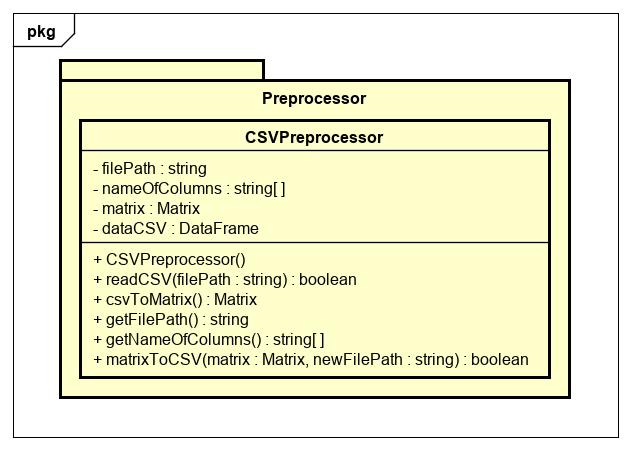
\includegraphics[scale=0.4]{preprocessorclassdiagram}
	\caption{Diagram kelas pada \textit{package Preprocessor}}
	\label{fig:preprocessorclassdiagram}
\end{figure}

\textit{Package Preprocessor} memiliki 3 buah kelas yang bertujuan untuk mengolah masukan perangkat lunak agar dapat diterapkan teknik \textit{Randomization}. Kelas tersebut yaitu \textit{CSVPreprocessor}, \textit{RotationMatrixPreprocessor}, dan \textit{ProjectionMatrixPreprocessor} yang akan dijelaskan secara detail pada subbab ini. Diagram kelas pada \textit{package Preprocessor} dapat dilihat pada Gambar~\ref{fig:preprocessorclassdiagram}.

\subsubsection{Kelas \textit{CSVPreprocessor}}
\label{subsubsec:kelas-csvpreprocessor}

Kelas \textit{CSVPreprocessor} berguna untuk mengolah masukan perangkat lunak yang berjenis \textit{comma-separated values} sebelum diterapkan teknik \textit{Randomization} agar masukan tersebut sesuai dengan persyaratan teknik \textit{Randomization}. Tujuan utama dari kelas ini adalah mengubah masukan berjenis \textit{comma-separated values} menjadi sebuah objek kelas \textit{Matrix} dan sebaliknya. Kelas ini memiliki tiga buah atribut dan enam buah fungsi yang selanjutnya akan dijelaskan secara rinci.

Berikut adalah deskripsi setiap atribut pada kelas \textit{CSVPreprocessor}.
\begin{itemize}
	\item \textit{filePath} adalah atribut untuk menyimpan lokasi masukan yang berjenis \textit{comma-separated values} yang ingin diolah pada komputer pengguna. Atribut ini memiliki tipe data \textit{string}.
	\item \textit{nameOfColumns} adalah atribut untuk menyimpan nama seluruh kolom pada dataset yang telah diolah. Atribut ini berupa array yang bertipe data \textit{string}.
	\item \textit{matrix} adalah atribut untuk menyimpan objek kelas \textit{Matrix} yang didapatkan dari hasil pengolahan masukan yang berjenis \textit{comma-separated values}. Atribut ini memiliki tipe data objek kelas \textit{Matrix}.
	\item \textit{dataCSV} adalah atribut untuk menyimpan data dokumen \textit{comma-separated values} yang telah dibaca dalam bentuk \textit{DataFrame}\footnote{https://pandas.pydata.org/pandas-docs/stable/reference/api/pandas.DataFrame.html}. Atribut ini memiliki tipe data objek kelas \textit{DataFrame}.
\end{itemize}

Berikut adalah deskripsi setiap fungsi pada kelas \textit{CSVPreprocessor}.
\begin{itemize}
	\item \textit{CSVPreprocessor} adalah \textit{constructor} kelas ini yang berfungsi untuk membuat sebuah objek kelas \textit{CSVPreprocessor} dan menginisialisasi semua atribut pada kelas ini. Fungsi ini tidak memiliki masukan apapun.
	\item \textit{readCSV} adalah fungsi untuk membaca dokumen berjenis \textit{comma-separated values} yang ingin diolah oleh kelas ini. Tujuan utama dari fungsi ini adalah menyimpan lokasi dokumen pada atribut \textit{filePath} dan menyimpan data dokumen \textit{comma-separated values} yang telah dibaca dalam bentuk \textit{DataFrame} pada atribut \textit{dataCSV}. Fungsi ini memiliki sebuah masukan bernama \textit{filePath} yang berguna untuk menentukan lokasi dokumen yang ingin diolah. Kembalian pada fungsi ini adalah sebuah \textit{boolean} yang menyatakan apakah fungsi ini berhasil membaca dokumen yang menjadi masukan fungsi \textit{readCSV}.
	\item \textit{csvToMatrix} adalah fungsi untuk mengolah dokumen \textit{comma-separated values} yang telah dibaca menjadi sebuah objek kelas \textit{Matrix}. Fungsi ini tidak memiliki masukan apapun tetapi mempunyai kembalian berupa objek kelas \textit{Matrix} yang didapatkan dari hasil pengolahan dokumen \textit{comma-separated values}.
	\item \textit{getFilePath} adalah fungsi untuk mendapatkan lokasi dokumen \textit{comma-separated values} yang telah dibaca atau dengan kata lain mendapatkan atribut \textit{filePath}. Fungsi ini tidak memiliki masukan apapun tetapi mempunyai kembalian berupa lokasi dokumen yang bertipe data \textit{string}.
	\item \textit{getNameOfColumns} adalah fungsi untuk mendapatkan nama semua kolom yang ada pada dokumen \textit{comma-separated values} yang telah dibaca atau dengan kata lain mendapatkan atribut \textit{nameOfColumns}. Fungsi ini tidak memiliki masukan apapun tetapi mempunyai kembalian berupa \textit{array} yang bertipe data \textit{string}.
	\item \textit{matrixToCSV} adalah fungsi untuk mengolah sebuah objek kelas \textit{Matrix} menjadi sebuah dokumen \textit{comma-separated values} atau dengan kata lain mengkonversi sebuah matriks menjadi dokumen berjenis \textit{comma-separated values}. Fungsi ini bisa dikatakan kebalikan dari fungsi \textit{csvToMatrix}. Ada dua buah masukan pada fungsi ini yaitu sebuah matriks dan lokasi penyimpanan dokumen yang baru. Kembalian pada fungsi ini adalah sebuah \textit{boolean} yang menyatakan apakah konversi berhasil dilakukan.
	\item \textit{getFileName} adalah fungsi untuk mendapatkan nama dokumen \textit{comma-separated values} yang telah dibaca. Fungsi ini tidak memiliki masukan apapun tetapi mempunyai kembalian berupa nama dokumen yang bertipe data \textit{string}.
\end{itemize}

\subsubsection{Kelas \textit{ProjectionMatrixPreprocessor}}
\label{subsubsec:kelas-projectionpre}

Kelas \textit{ProjectionMatrixPreprocessor} berguna untuk mengolah masukan perangkat lunak berupa matriks proyeksi yang berjenis \textit{comma-separated values} sebelum diterapkan teknik \textit{Randomization} agar masukan tersebut sesuai dengan persyaratan teknik \textit{Randomization}. Tujuan utama dari kelas ini adalah mengubah masukan matriks proyeksi berjenis \textit{comma-separated values} menjadi sebuah objek kelas \textit{Matrix} dan sebaliknya. Kelas ini memiliki sebuah atribut dan tiga buah fungsi yang selanjutnya akan dijelaskan secara rinci.

Berikut adalah deskripsi setiap atribut pada kelas \textit{ProjectionMatrixPreprocessor}.
\begin{itemize}
	\item \textit{projectionMatrix} adalah atribut untuk menyimpan matriks proyeksi yang berbentuk objek kelas \textit{Matrix} yang didapatkan dari hasil pengolahan masukan yang berjenis \textit{comma-separated values}. Atribut ini memiliki tipe data objek kelas \textit{Matrix}.
\end{itemize}

Berikut adalah deskripsi setiap fungsi pada kelas \textit{ProjectionMatrixPreprocessor}.
\begin{itemize}
	\item \textit{readFromCSV} adalah fungsi untuk membaca dokumen berjenis \textit{comma-separated values} menjadi matriks proyeksi yang dapat dipakai perangkat lunak. Fungsi ini memiliki sebuah masukan bernama \textit{filePath} yang berguna untuk menentukan lokasi dokumen yang ingin diolah. Kembalian pada fungsi ini adalah sebuah \textit{boolean} yang menyatakan apakah pembacaan dokumen berhasil dilakukan.
	\item \textit{saveToCSV} adalah fungsi statis untuk mengolah sebuah matriks proyeksi berbentuk objek kelas \textit{Matrix} menjadi sebuah dokumen \textit{comma-separated values} dan menyimpannya pada sebuah direktori pengguna. Fungsi ini bisa dikatakan kebalikan dari fungsi \textit{readFromCSV}. Ada dua buah masukan pada fungsi ini yaitu sebuah matriks proyeksi dan lokasi penyimpanan dokumen yang baru. Kembalian pada fungsi ini adalah sebuah \textit{boolean} yang menyatakan apakah penyimpanan berhasil dilakukan.
	\item \textit{getProjectionMatrix} adalah fungsi untuk mendapatkan matriks proyeksi berbentuk objek kelas \textit{Matrix} yang didapatkan dari fungsi \textit{readFromCSV} atau dengan kata lain mendapatkan variabel \textit{projectionMatrix}. Fungsi ini tidak memiliki masukan apapun tetapi mempunyai kembalian berupa matriks proyeksi yang bertipe data \textit{Matrix}.
\end{itemize}

\subsubsection{Kelas \textit{RotationMatrixPreprocessor}}
\label{subsubsec:kelas-rotationpre}

Kelas \textit{RotationMatrixPreprocessor} berguna untuk mengolah masukan perangkat lunak berupa matriks rotasi dan translasi yang berjenis \textit{comma-separated values} sebelum diterapkan teknik \textit{Randomization} agar masukan tersebut sesuai dengan persyaratan teknik \textit{Randomization}. Tujuan utama dari kelas ini adalah mengubah masukan matriks rotasi dan translasi berjenis \textit{comma-separated values} menjadi dua buah objek kelas \textit{Matrix} dan sebaliknya. Kelas ini memiliki dua buah atribut dan empat buah fungsi yang selanjutnya akan dijelaskan secara rinci.

Berikut adalah deskripsi setiap atribut pada kelas \textit{RotationMatrixPreprocessor}.
\begin{itemize}
	\item \textit{rotationMatrix} adalah atribut untuk menyimpan matriks rotasi yang berbentuk objek kelas \textit{Matrix} yang didapatkan dari hasil pengolahan masukan yang berjenis \textit{comma-separated values}. Atribut ini memiliki tipe data objek kelas \textit{Matrix}.
	\item \textit{translationMatrix} adalah atribut untuk menyimpan matriks translasi yang berbentuk objek kelas \textit{Matrix} yang didapatkan dari hasil pengolahan masukan yang berjenis \textit{comma-separated values}. Atribut ini memiliki tipe data objek kelas \textit{Matrix}.
\end{itemize}

Berikut adalah deskripsi setiap fungsi pada kelas \textit{RotationMatrixPreprocessor}.
\begin{itemize}
	\item \textit{readFromCSV} adalah fungsi untuk membaca dokumen berjenis \textit{comma-separated values} menjadi matriks rotasi dan translasi yang dapat dipakai perangkat lunak. Fungsi ini memiliki sebuah masukan bernama \textit{filePath} yang berguna untuk menentukan lokasi dokumen yang ingin diolah. Kembalian pada fungsi ini adalah sebuah \textit{boolean} yang menyatakan apakah pembacaan dokumen berhasil dilakukan.
	\item \textit{saveToCSV} adalah fungsi statis untuk mengolah sebuah matriks rotasi dan translasi berbentuk objek kelas \textit{Matrix} menjadi sebuah dokumen \textit{comma-separated values} dan menyimpannya pada sebuah direktori pengguna. Fungsi ini bisa dikatakan kebalikan dari fungsi \textit{readFromCSV}. Ada tiga buah masukan pada fungsi ini yaitu sebuah matriks rotasi, matriks translasi dan lokasi penyimpanan dokumen yang baru. Kembalian pada fungsi ini adalah sebuah \textit{boolean} yang menyatakan apakah penyimpanan berhasil dilakukan.
	\item \textit{getRotationMatrix} adalah fungsi untuk mendapatkan matriks rotasi berbentuk objek kelas \textit{Matrix} yang didapatkan dari fungsi \textit{readFromCSV} atau dengan kata lain mendapatkan variabel \textit{rotationMatrix}. Fungsi ini tidak memiliki masukan apapun tetapi mempunyai kembalian berupa matriks rotasi yang bertipe data \textit{Matrix}.
	\item \textit{getTranslationMatrix} adalah fungsi untuk mendapatkan matriks translasi berbentuk objek kelas \textit{Matrix} yang didapatkan dari fungsi \textit{readFromCSV} atau dengan kata lain mendapatkan variabel \textit{translationMatrix}. Fungsi ini tidak memiliki masukan apapun tetapi mempunyai kembalian berupa matriks translasi yang bertipe data \textit{Matrix}.
\end{itemize}

\section{Masukan Perangkat Lunak}
\label{sec:masukan-pl}

Perangkat lunak akan mempunyai sebuah masukan yang berupa dataset. Dataset yang ingin diacak memiliki persyaratan yaitu harus berupa sebuah matriks. Tetapi mayoritas dataset yang ada didistribusikan bukan sebagai matriks melainkan dokumen berjenis tertentu antara lain seperti dokumen berjenis \textit{comma-separated values}. Oleh karena itu, perangkat lunak ini hanya dapat menerima masukan berupa dokumen berjenis \textit{comma-separated values}. Berikut akan dijelaskan secara rinci masukan yang dapat diterima oleh perangkat lunak.

Dokumen \textit{comma-separated values} adalah dokumen berisi teks yang menggunakan koma untuk memisahkan antara tiap nilai dengan nilai lainnya. Berikut adalah contoh isi dari dokumen berjenis \textit{comma-separated values}.
\begin{verbatim}
	sepal_length,sepal_width,petal_length,petal_width,species
	5.1,3.5,1.4,0.2,setosa
	4.9,3,1.4,0.2,setosa
	4.7,3.2,1.3,0.2,setosa
	4.6,3.1,1.5,0.2,setosa
	5,3.6,1.4,0.2,setosa
	5.4,3.9,1.7,0.4,setosa
	4.6,3.4,1.4,0.3,setosa
	5,3.4,1.5,0.2,setosa
	4.4,2.9,1.4,0.2,setosa
	4.9,3.1,1.5,0.1,setosa
\end{verbatim}
Baris pertama pada contoh di atas merupakan nama semua kolom yang ada pada dataset. Baris lainnya adalah nilai-nilai setiap kolom pada suatu rekord. Pada dataset di atas, kolom terakhir adalah kolom label. Selain kolom tersebut adalah kolom fitur yang akan diacak. Kolom fitur tersebut untuk perangkat lunak \textit{Randomization} ini mempunyai persyaratan yaitu nilai kolom tersebut harus berjenis numerik.
